\documentclass[a4paper,11pt]{article}
\usepackage{setspace}
\onehalfspacing
  
\usepackage{caption}
\usepackage{titlesec}
\usepackage{graphicx}
\usepackage{listings}
\usepackage{xcolor}
\usepackage{fancyhdr}
\usepackage[a4paper,margin=1in]{geometry}
\usepackage{mdframed} %nice frames

\definecolor{light-gray}{gray}{0.95} %the shade of grey that stack exchange uses

\renewcommand{\thispagestyle}[1]{} % do nothing

\lstset{
  language=Python,
  aboveskip=3mm,
  belowskip=3mm,
  showstringspaces=true,
  columns=flexible,
  basicstyle={\small\ttfamily},
  numbers=none,
  numberstyle=\tiny\color{gray},
  keywordstyle=\color{blue},
  commentstyle=\color{red},
  breaklines=true,
  breakatwhitespace=true,
  tabsize=2
}

\graphicspath{ {./images/} }
\titlespacing{\section}{0pc}{1pc}{1pc}
 
\pagestyle{fancy}
\fancyhf{}
\rhead{Assignment 6}
\lhead{Programming using libpcap}
\rfoot{Page \thepage}

 
\begin{document}
\title{\vspace{-1.0cm}\textbf{Programming using libpcap}}
\author{
  \textbf{Tan Wei Xuan (49003140)}\\
  \texttt{tanweixuan@postech.ac.kr}
}
\date{\today}
\maketitle

\section{Installing Dependencies}
Ensure that all dependencies are installed on the operating system. The operating system that I am using is \textbf{Ubuntu 18.04.2 bit subsystem} and the list of required dependencies are as listed below:
\begin{enumerate}
\item \textbf{GCC}
\item \textbf{build-essential}
\item \textbf{libpcap}

\subsection{Installing GCC}
The following linux command will install the \textbf{GCC compiler} on on Ubuntu 18.04. Open up terminal and enter:
\begin{mdframed}[backgroundcolor=light-gray, roundcorner=30pt,leftmargin=1, rightmargin=1, innerleftmargin=5, innertopmargin=-3,innerbottommargin=5, outerlinewidth=1, linecolor=light-gray]
\begin{lstlisting}
$ sudo apt install g++
\end{lstlisting}
\end{mdframed}
\subsection{Installing build-essential}
The following linux command will install the \textbf{build-essential} package on on Ubuntu 18.04. Open up terminal and enter:
\begin{mdframed}[backgroundcolor=light-gray, roundcorner=30pt,leftmargin=1, rightmargin=1, innerleftmargin=5, innertopmargin=-3,innerbottommargin=5, outerlinewidth=1, linecolor=light-gray]
\begin{lstlisting}
$ sudo apt install build-essential
\end{lstlisting}
\end{mdframed}
\subsection{Installing libpcap}
The following linux command will install the \textbf{libpcap} package on on Ubuntu 18.04. Open up terminal and enter:
\begin{mdframed}[backgroundcolor=light-gray, roundcorner=30pt,leftmargin=1, rightmargin=1, innerleftmargin=5, innertopmargin=-3,innerbottommargin=5, outerlinewidth=1, linecolor=light-gray]
\begin{lstlisting}
$ sudo apt install libpcap-dev
\end{lstlisting}
\end{mdframed}
\end{enumerate}

\section{Capturing Packets using libpcap}
The file \textbf{"question1.cpp"} contains the source code required to capture \textbf{TCP, UDP and ICMP traffic} on my Network Interface Card for a period of 40 seconds. The key functions that I have utilised to capture these traffic are as follow:
\begin{enumerate}
\item \textbf{pcap\_lookupdev()}
\newline This function finds a default network device on which to capture packets from
\item \textbf{pcap\_openlive()}
\newline This function is used to establish a connection with the network device that can bring packets
\item \textbf{pcap\_compile() and pcap\_setfilter()}
\newline These functions are used to filter and capture only \textbf{TCP, UDP and ICMP} paclets which go through the well-known ports (1 ~ 1024).
\item \textbf{pcap\_dump\_open() and pcap\_dump}
pcap\_dump\_open() opens a dump file to output and pcap\_dump prints a packet to the dump file created.
\end{enumerate}
\noindent 
In order to compile the source code (question1.cpp), we need to run the following command.
\vspace*{-\baselineskip} 
\begin{mdframed}[backgroundcolor=light-gray, roundcorner=30pt,leftmargin=1, rightmargin=1, innerleftmargin=5, innertopmargin=-3,innerbottommargin=5, outerlinewidth=1, linecolor=light-gray]
\begin{lstlisting}
$ gcc question1.c -lpcap
\end{lstlisting}
\end{mdframed}
In order to execute our program, we have to run the following command.
\begin{mdframed}[backgroundcolor=light-gray, roundcorner=30pt,leftmargin=1, rightmargin=1, innerleftmargin=5, innertopmargin=-3,innerbottommargin=5, outerlinewidth=1, linecolor=light-gray]
\begin{lstlisting}
$sudo ./a.out <argument1> <argument2>
\end{lstlisting}
\end{mdframed}
The program expects the following two arguments:
\begin{enumerate}
\item \textbf{$\langle$Argument 1$\rangle$}
\newline The first argument is the period to capture in seconds. 
\item \textbf{$\langle$Argument 2$\rangle$}
\newline The second argument is the name of the output file to print the captured packets to.
\end{enumerate}
The following command will generate the output file containg the captured packets.
\begin{figure}[h!]
	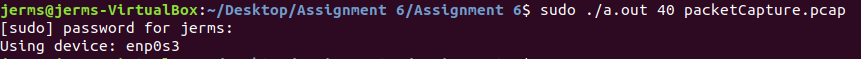
\includegraphics[width = 16cm]{question1}
	\caption{\textit{Executing question1.cpp}}
\end{figure}
\newline
My packet capture file is provided in \textbf{packetCapture.pcap}. The time period of capture is \textbf{40 seconds}.

\section{Packet Analysis using libpcap}
The file \textbf{"question2.cpp"} contains the source code required to capture \textbf{TCP, UDP and ICMP traffic} on my Network Interface Card and to print out the different traffic traces analysis results for the captued packets. The key steps and functionality of my code are as listed below:
\newline \newline
\noindent Firstly, we will open our previously captured file for offline processing with the command \textbf{pcap\_open\_offline()}
\begin{mdframed}[backgroundcolor=light-gray, roundcorner=30pt,leftmargin=1, rightmargin=1, innerleftmargin=5, innertopmargin=-3,innerbottommargin=5, outerlinewidth=1, linecolor=light-gray]
\begin{lstlisting}
if((file = pcap_open_offline(argv[1], error_buffer)) == NULL) {
			printf("pcap_open_offline() failed.\n%s\n", error_buffer);
			exit(1);
}
\end{lstlisting}
\end{mdframed}
Next, we parse through each packet till the end with the function \textbf{pcap\_next}. 
\begin{mdframed}[backgroundcolor=light-gray, roundcorner=30pt,leftmargin=1, rightmargin=1, innerleftmargin=5, innertopmargin=-3,innerbottommargin=5, outerlinewidth=1, linecolor=light-gray]
\begin{lstlisting}
while((packet = pcap_next(file, &header)) != NULL) {
	//Code not included for this portion
}
\end{lstlisting}
\end{mdframed}
Wiithin the loop, for each packet, we perform traffic analysis through the following steps:
\begin{enumerate}
\item \textbf{Record timestamp of packet}
\newline The timestamp for each packet is recorded. The timestamp and length of the packet can be found in the libpcap header.
\begin{mdframed}[backgroundcolor=light-gray, roundcorner=30pt,leftmargin=1, rightmargin=1, innerleftmargin=5, innertopmargin=-3,innerbottommargin=5, outerlinewidth=1, linecolor=light-gray]
\begin{lstlisting}
if(total_packets == 1) {
			time_first = header.ts.tv_sec * 1000000 + header.ts.tv_usec;
}
time_last = header.ts.tv_sec * 1000000 + header.ts.tv_usec;
\end{lstlisting}
\end{mdframed}
\item \textbf{Analyse which Transport Layer Protocol is used}
\newline We perform an analysis on which transport layer protocol is being used (TCP, UDP or ICMP) by adding an offset of 0x17 to the packet.
\begin{mdframed}[backgroundcolor=light-gray, roundcorner=30pt,leftmargin=1, rightmargin=1, innerleftmargin=5, innertopmargin=-3,innerbottommargin=5, outerlinewidth=1, linecolor=light-gray]
\begin{lstlisting}
switch(*(packet + 0x17)) {
			case 0x01: cnt_icmp++; break;
			case 0x06: cnt_tcp++; break;
			case 0x11: cnt_udp++; break;
			default: break;
}
\end{lstlisting}
\end{mdframed}
\item \textbf{Analyse number of Packets of FTP, SSH, DNS and HTTP}
We perform an analysis on the number of packets of FTP, SSH, DNS and HTTP by adding an offset of \textbf{0x22 - 0x23} and \textbf{0x24 - 0x25} to the packet to get the source and destination port respectively. As FTP uses port 21, SSH uses port 22, DNS uses port 53 and HTTP uses port 80,  depending on the value of the source or destination port, we can categorise the traffic into either FTP, SSH, DNS or HTTP.
\begin{mdframed}[backgroundcolor=light-gray, roundcorner=30pt,leftmargin=1, rightmargin=1, innerleftmargin=5, innertopmargin=-3,innerbottommargin=5, outerlinewidth=1, linecolor=light-gray]
\begin{lstlisting}
src_port = *(packet + 0x22) * 256 + *(packet + 0x23);
dest_port = *(packet + 0x24) * 256 + *(packet + 0x25);
if(src_port == 21 || dest_port == 21) cnt_ftp++;
	else if(src_port == 22 || dest_port == 22) cnt_ssh++;
	else if(src_port == 53 || dest_port == 53) cnt_dns++;
	else if(src_port == 80 || dest_port == 80) cnt_http++;
\end{lstlisting}
\end{mdframed}
\item \textbf{Update Endhost List} 
\newline When we reach an end's IP address, we update the endhost list. The endhost list is implemented as a linked list such that if an IP address has being used previously, it will update the packet count and total bytes to that node. Otherwise, it will create a new node at the end of the list with the new IP address. We use an offset of 0xb and 0xe to add the destination and source IPs to the endhost list respectively.
\begin{mdframed}[backgroundcolor=light-gray, roundcorner=30pt,leftmargin=1, rightmargin=1, innerleftmargin=5, innertopmargin=-3,innerbottommargin=5, outerlinewidth=1, linecolor=light-gray]
\begin{lstlisting}
update_endhost(packet + 0xb, &hosts, header.len);
update_endhost(packet + 0xe, &hosts, header.len);
\end{lstlisting}
\end{mdframed}
\end{enumerate}
We can compile the source code (question2.cpp) the same way as we did previously.
\begin{mdframed}[backgroundcolor=light-gray, roundcorner=30pt,leftmargin=1, rightmargin=1, innerleftmargin=5, innertopmargin=-3,innerbottommargin=5, outerlinewidth=1, linecolor=light-gray]
\begin{lstlisting}
$ gcc question2.c -lpcap
\end{lstlisting}
\end{mdframed}
In order to execute our program, we have to run the following command.
\begin{mdframed}[backgroundcolor=light-gray, roundcorner=30pt,leftmargin=1, rightmargin=1, innerleftmargin=5, innertopmargin=-3,innerbottommargin=5, outerlinewidth=1, linecolor=light-gray]
\begin{lstlisting}
$sudo ./a.out <argument1> <argument2>
\end{lstlisting}
\end{mdframed}
The program expects the following two arguments:
\begin{enumerate}
\item \textbf{$\langle$Argument 1$\rangle$}
\newline The first argument is name of the packet capture file to perform analysis on. For my assignment, the name of the file is \textbf{packetCapture.pcap}.
\item \textbf{$\langle$Argument 2$\rangle$}
\newline The second argument is the name of the output file to print the endpoint analysis to. This file will contain the total number of pakcets and total number of bytes for each endpoint IP Address. For my assignment, the name of the output file is \textbf{endpointAnalysis.txt}.
\end{enumerate}
The following command will generate the output file containg the endpoint analysis of the provided packet capture file.
\newline
\begin{figure}[h!]
	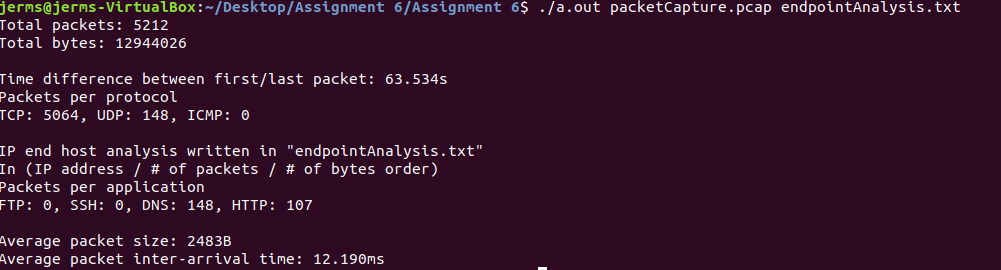
\includegraphics[width = 16cm]{question2}
	\caption{\textit{Executing question2.cpp}}
\end{figure}
\newline
The endpoint analysis (the number of packet and total bytes of each end host) is provided in \textbf{endpointAnalysis.txt}. Other required categories of analyzed data are shown in Figure 2 above. The categories of analyzed data will be printed out on the terminal upon execution of the program.

\section{Packet Decapsulation using libpcap}
The file \textbf{"question3.cpp"} contains the source code required to perform packet decapsulation of the given trace file. The implementation of the packet decapsulation are similar to \textit{"question2.cpp"}, however, in order to know what is inside the IP packet that is encapsulated by the GTP protocol,  a few minor changes (listed below)  have been made to the code:
\begin{enumerate}
\item \textbf{Obtaining Inner Packet's Length}
\newline 
Every packet in the provided trace file has two IP headers: The original one (outer packet) and another one within the GTP protocol (inner packet). The data outside the Inner Packet is 40 bytes, with 36 bytes being on the front and 4 bytes of Ethernet protocol footer at the back. Therefore, we can simply subtract 40 from the Outer Packet's length to obtain the Inner Packet's length.
\begin{mdframed}[backgroundcolor=light-gray, roundcorner=30pt,leftmargin=1, rightmargin=1, innerleftmargin=5, innertopmargin=-3,innerbottommargin=5, outerlinewidth=1, linecolor=light-gray]
\begin{lstlisting}
total_bytes += (header.len - 40);
\end{lstlisting}
\end{mdframed}
\item \textbf{Accessing Inner Packet}
\newline
For each packet, the offset difference between the Inner and Outer Packet is constant and thus we can simply add 40 to the packet pointer to access the Inner Packet.
\begin{mdframed}[backgroundcolor=light-gray, roundcorner=30pt,leftmargin=1, rightmargin=1, innerleftmargin=5, innertopmargin=-3,innerbottommargin=5, outerlinewidth=1, linecolor=light-gray]
\begin{lstlisting}
while((packet = pcap_next(file, &header)) != NULL) {
	packet += 0x28;
}
\end{lstlisting}
\end{mdframed}
\end{enumerate}

We can compile the source code (question3.cpp) the same way as we did previously.
\begin{mdframed}[backgroundcolor=light-gray, roundcorner=30pt,leftmargin=1, rightmargin=1, innerleftmargin=5, innertopmargin=-3,innerbottommargin=5, outerlinewidth=1, linecolor=light-gray]
\begin{lstlisting}
$ gcc question3.c -lpcap
\end{lstlisting}
\end{mdframed}
In order to execute our program, we have to run the following command.
\begin{mdframed}[backgroundcolor=light-gray, roundcorner=30pt,leftmargin=1, rightmargin=1, innerleftmargin=5, innertopmargin=-3,innerbottommargin=5, outerlinewidth=1, linecolor=light-gray]
\begin{lstlisting}
$sudo ./a.out <argument1> <argument2>
\end{lstlisting}
\end{mdframed}
The program expects the following two arguments:
\begin{enumerate}
\item \textbf{$\langle$Argument 1$\rangle$}
\newline The first argument is name of the packet capture file to perform analysis on. We will be utilising the provided packet capture file, \textbf{internet\_trace.pcap}.
\item \textbf{$\langle$Argument 2$\rangle$}
\newline The second argument is the name of the output file to print the endpoint analysis to. This file will contain the total number of pakcets and total number of bytes for each endpoint IP Address. For my assignment, the name of the output file is \textbf{internetTrace\_endpointAnalysis.txt}.
\end{enumerate}
The following command will generate the output file containg the endpoint analysis of the provided packet capture file.
\newline
\begin{figure}[h!]
	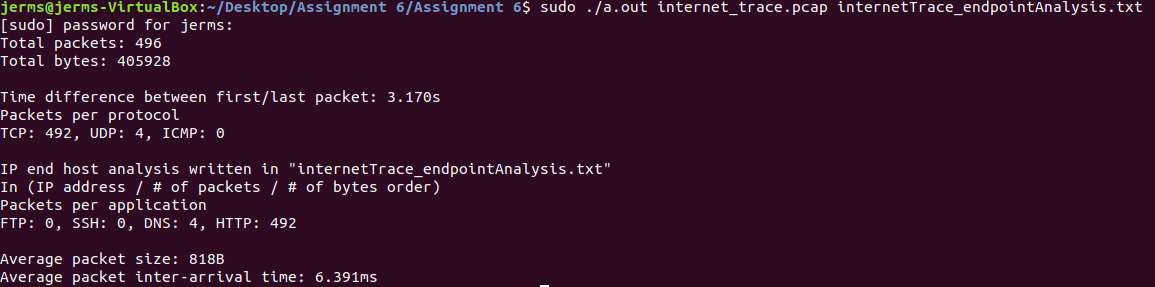
\includegraphics[width = 16cm]{question3}
	\caption{\textit{Executing question3.cpp}}
\end{figure}
\newline
The endpoint analysis (the number of packet and total bytes of each end host) is provided in \textbf{internetTrace\_endpointAnalysis.txt}. Other required categories of analyzed data are shown in Figure 3 above. The categories of analyzed data will be printed out on the terminal upon execution of the program.
\end{document}